\documentclass[mathserif]{beamer}

\useoutertheme{split}
\useinnertheme{rectangles}
\usecolortheme{uiuc}
\logo{
\includegraphics[height=0.5cm]{uiuclogo.pdf}}

\usepackage{beamerthemesplit} % TODO: use different beamer theme
\usepackage{framed}
%\usepackage{amsmath}

\title{SIAM: Getting Started with \LaTeX}
\author{Matthew Michelotti}
\date{\today}

\renewcommand{\arraystretch}{1.1}

\setbeamertemplate{navigation symbols}{}%remove navigation symbols
\setbeamertemplate{caption}[numbered]

\begin{document}

\defbeamertemplate*{footline}{shadow theme} {
\leavevmode \hbox{\begin{beamercolorbox}[wd=.5\paperwidth,
ht=2.5ex,dp=1.125ex,leftskip=.3cm plus1fill,rightskip=.3cm]
{author in head/foot}%
\usebeamerfont{author in head/foot}\insertshortauthor
\end{beamercolorbox}\begin{beamercolorbox}[wd=.5\paperwidth,
ht=2.5ex,dp=1.125ex,leftskip=.3cm,rightskip=.3cm plus1fil]
{title in head/foot}%
\usebeamerfont{title in head/foot}\insertshorttitle
\hfill \insertframenumber{} / \inserttotalframenumber
\end{beamercolorbox}}
}

\frame{\titlepage}

\begin{frame}[fragile]
  \frametitle{What is \LaTeX{}?}

  \begin{itemize}
  \item \LaTeX{} is a high-quality typesetting system
  \item \LaTeX{} markup is converted into nice looking pdf files
  \end{itemize}

  \begin{minipage}{.38\textwidth}
  \begin{framed}
    \tiny
    \begin{verbatim}\documentclass[12pt]{article}
\usepackage{amsmath}
\title{\LaTeX}
\date{}
\begin{document}
  \maketitle
  \section{Introduction}
  \LaTeX{} is a document
  preparation system for the
  \TeX{} typesetting program.
  It offers programmable desktop
  publishing features and
  ...
  \begin{align}
    E &= mc^2 \\
    m &= \frac{m_0}
      {\sqrt{1-\frac{v^2}{c^2}}}
  \end{align}
\end{document}\end{verbatim}
  \end{framed}
  \end{minipage}
  $\rightarrow$
  \begin{minipage}{.55\textwidth} 
  \begin{framed}
    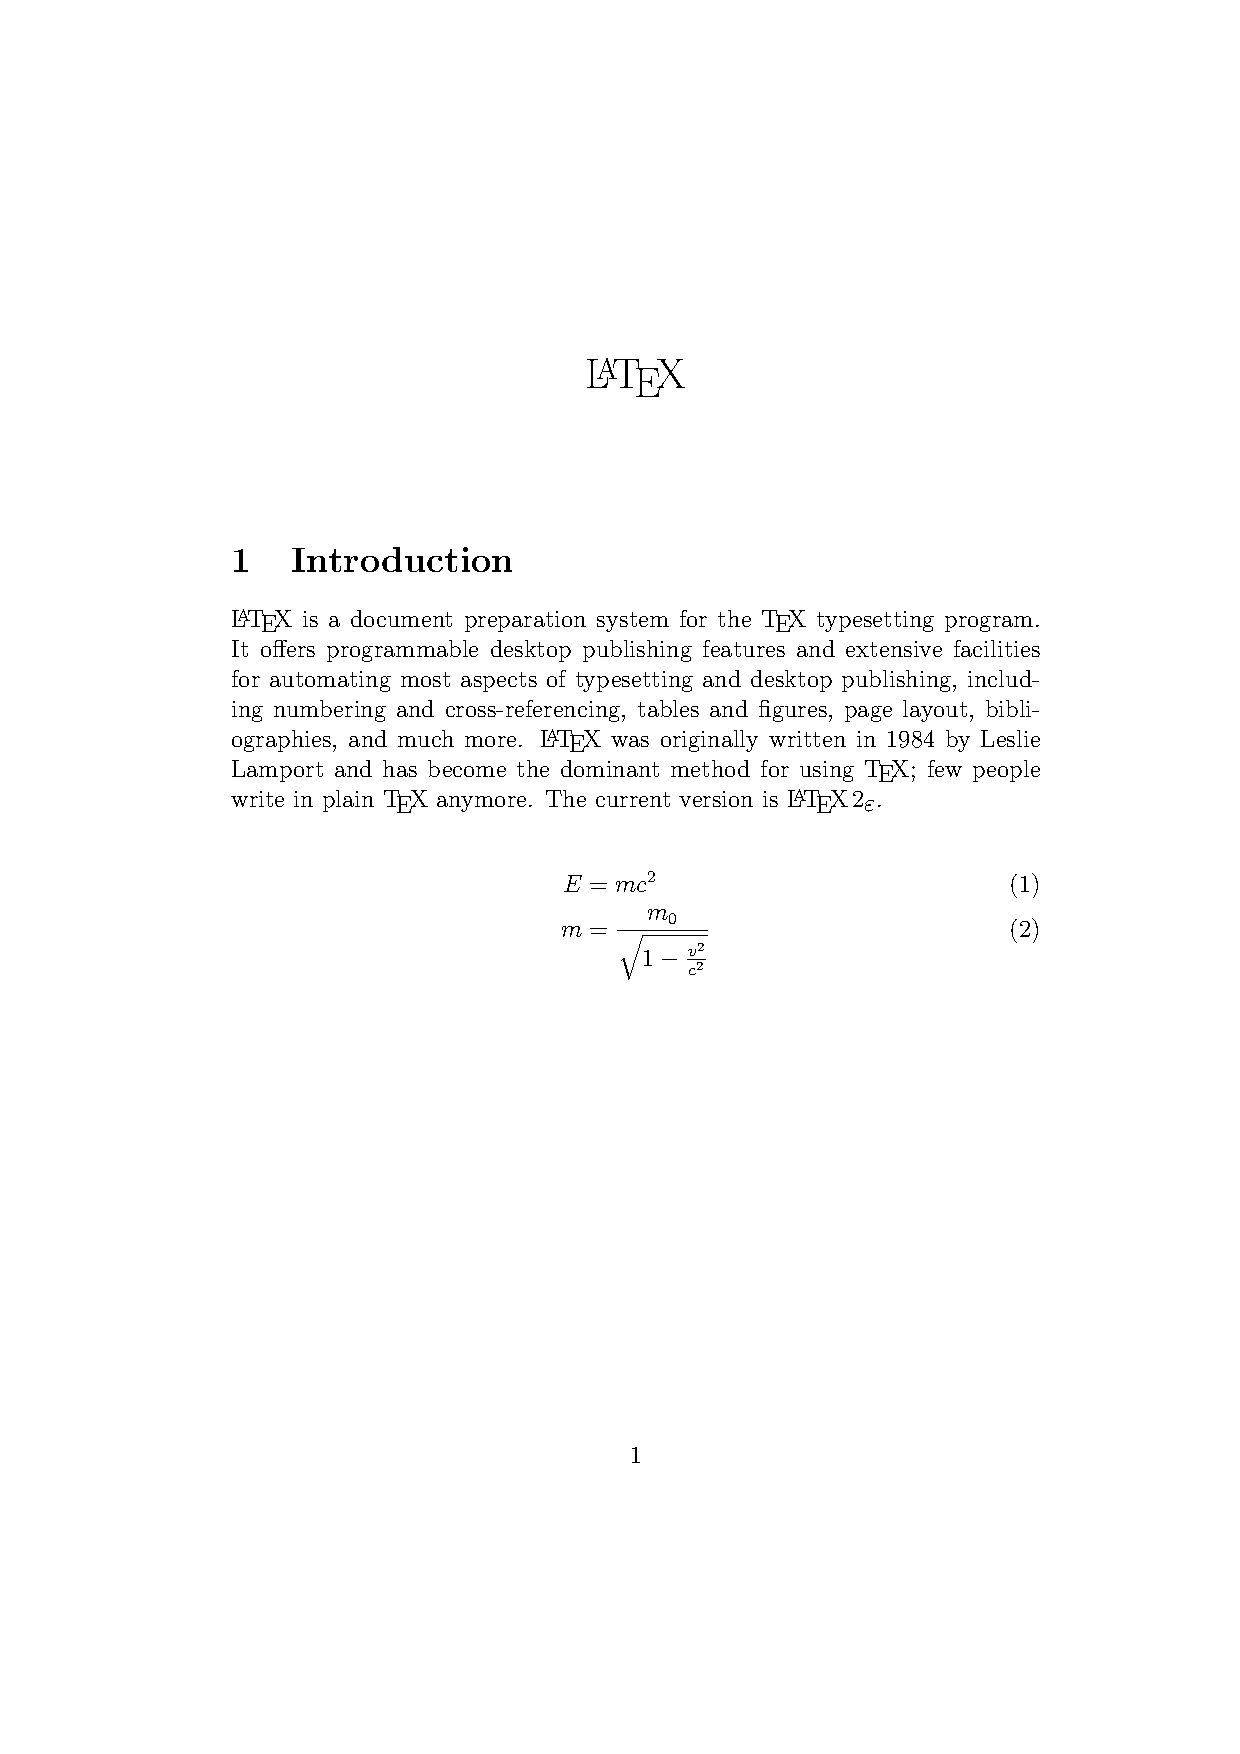
\includegraphics[trim = 33mm 127mm 33mm 59mm, clip, width=\textwidth]{figures/example_article.pdf}
  \end{framed}
  \end{minipage}
\end{frame}

\begin{frame}[fragile]
  \frametitle{Why Use \LaTeX{}?}
  \begin{itemize}
    \item Produces high-quality documents
    \item Offers precise control over how document looks
    \item Excellent for typesetting mathematics
    \item Automated references, citations, etc.
    \item Used for papers, r\'esum\'es, presentation slides, etc.
    \item Widely used for academic journals
    \item Free
    \item Multi-platform
  \end{itemize}
\end{frame}

\begin{frame}[fragile]
  \frametitle{Compiling}
  \begin{itemize}
  \item Installing \LaTeX{} on your computer
  \begin{itemize}
    \item Mac: from MacPorts, MacTeX, TeXShop
    \item Windows: TeXworks, MiKTeX
    \item Helpful site: en.wikibooks.org/wiki/LaTeX/Installation
  \end{itemize}
  \item Use \verb|latexmk| or \verb|pdflatex| or \verb|latex| command on a .tex file to produce output
  \begin{itemize}
    \item \verb|latex| command is not recommended, since it cannot include .pdf, .jpg, .png image formats
      and cannot output to .pdf
  \end{itemize}
  \item Can also compile online at sharelatex.com
  \end{itemize}
  \begin{figure}
  
\includegraphics[width=.2\textwidth]{figures/texshop.png} \quad
  
\includegraphics[width=.22\textwidth]{figures/texworks.png} \quad
  
\includegraphics[width=.2\textwidth]{figures/share_latex.jpg}
  \end{figure}
\end{frame}

%\frame{
%  \frametitle{Exercise 1: Compiling}
%  \begin{itemize}
%    \item If you have \LaTeX{} installed on your laptop, you can use that
%    \item Otherwise, go to www.compileonline.com/try\_latex\_online.php
%    \item Compile the example \LaTeX{} file on this website
%    \begin{itemize} \item The result should look as follows: \end{itemize}
%  \end{itemize}
%
%  \centerline{
%  \begin{minipage}{.6\textwidth} 
%  \begin{framed}
%    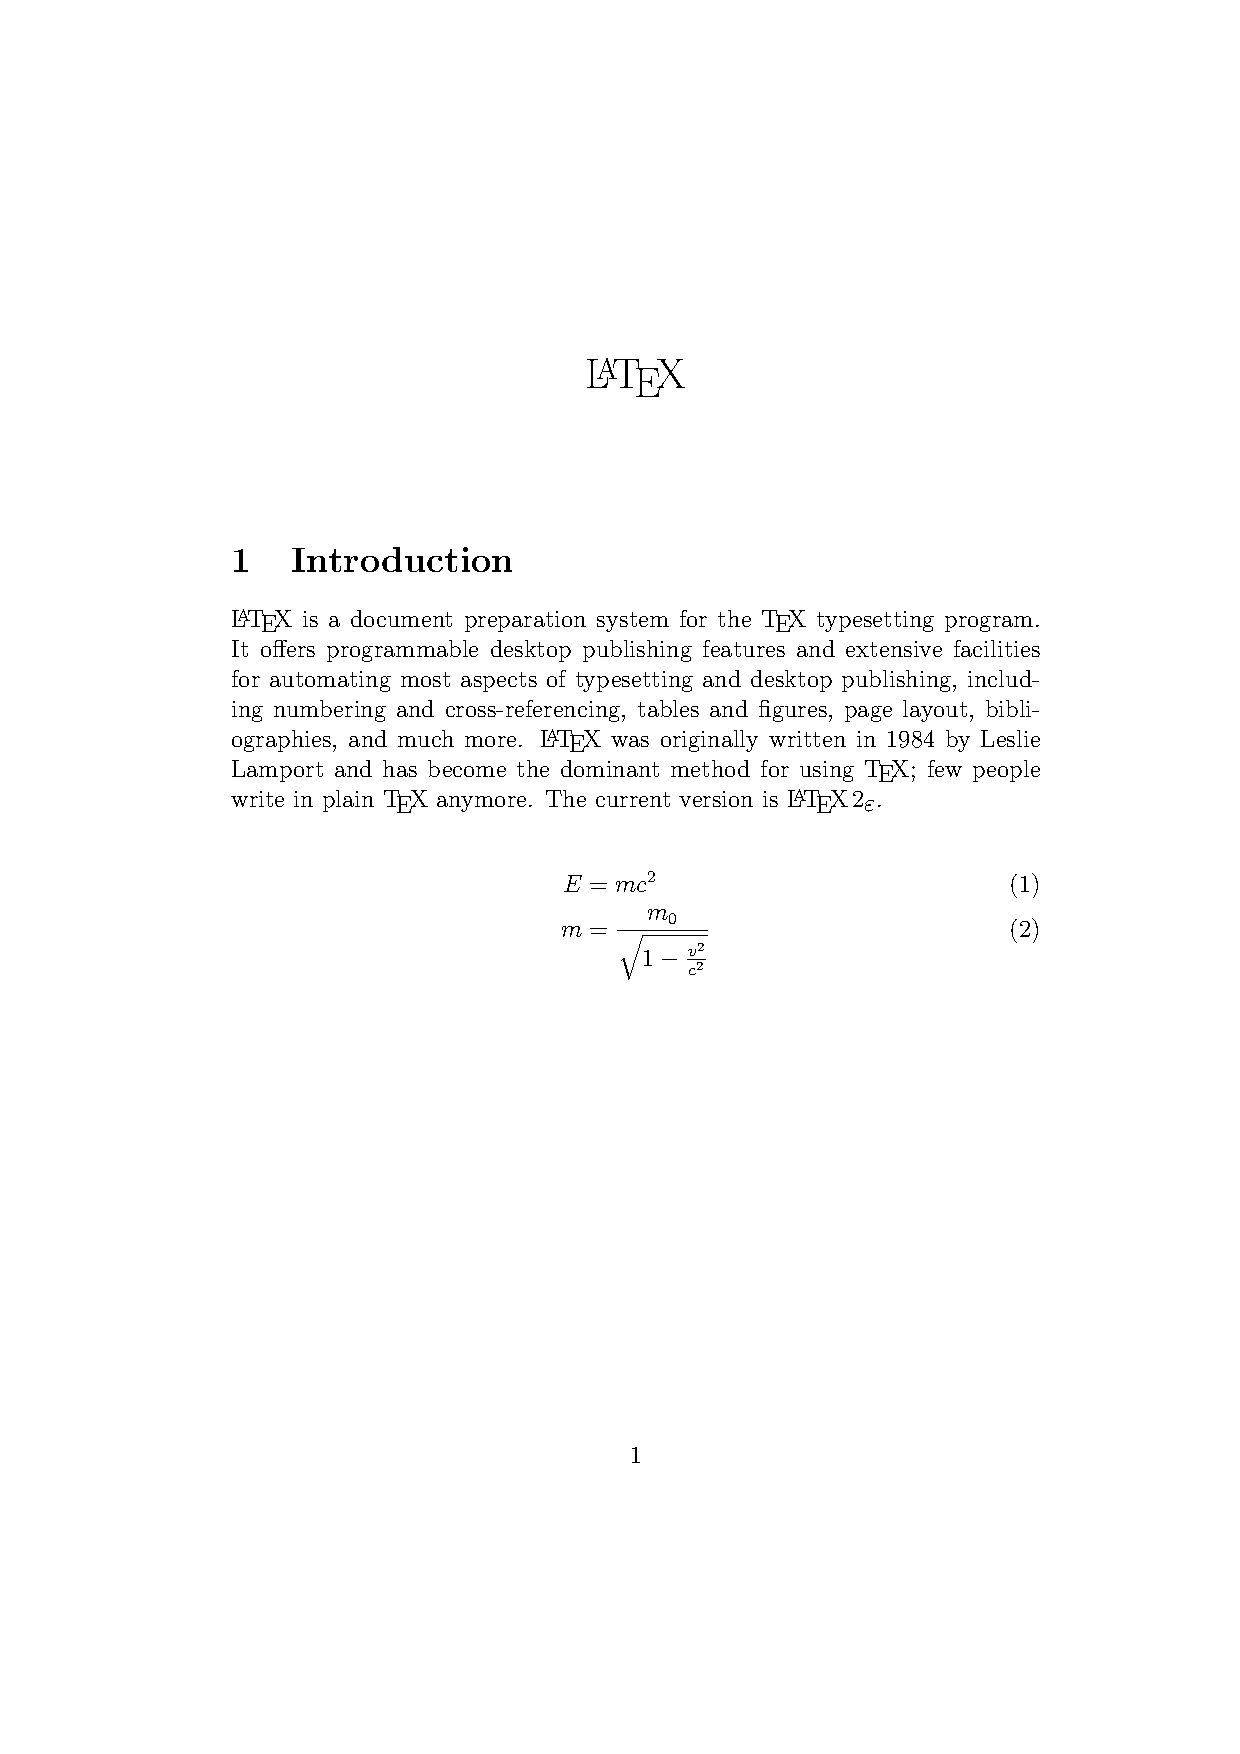
\includegraphics[trim = 33mm 127mm 33mm 59mm, clip, width=\textwidth]{figures/example_article.pdf}
%  \end{framed}
%  \end{minipage}
%  }
%}

\begin{frame}[fragile]
  \frametitle{Control Sequences}
  \begin{itemize}
    \item \LaTeX{} uses control sequences to achieve special functionality
    \item Control sequences start with a backslash \verb|\|
  \end{itemize}
  \small
  \begin{table}
  \begin{tabular}{l l}
    \verb|\documentclass[11pt]{article}| & describes appearance of document \\
     & (similar to CSS) \\
    \verb|\usepackage{amsmath}| & include package named amsmath \\
    \verb|\begin{document}| & begins document environment \\
    \verb|\section{Section Title}| & starts a new section \\
    \verb|\subsection{Subsection Title}| & starts a new subsection \\
    \verb|\LaTeX{}| & displays \LaTeX{} \\
    \verb|\end{document}| & ends document environment
  \end{tabular}
  \end{table}
\end{frame}

\begin{frame}[fragile]
  \frametitle{Example Document}
  \begin{itemize}
    \item \LaTeX{} document will have information like package imports, title and date 
    in preamble and top matter
    \item Contents of document belong in document environment
  \end{itemize}
  \begin{verbatim}\documentclass[11pt]{article}
\usepackage{amsmath}
\title{\LaTeX}
\author{Your Name}
\date{} % omits date since this is empty
\begin{document}
  \maketitle
  \section{Introduction}
  This is the introduction of my document.
  ...
\end{document}\end{verbatim}
\end{frame}

\begin{frame}[fragile]
  \frametitle{Spaces and Quotes}
{\small
\begin{verbatim}You can use LaTeX to typeset regular text.  In LaTeX, using
extra     spaces       or      a newline   doesn't matter.

However, using two newlines in a row results in a new
paragraph.
``This sentence is quoted.''

% line comments begin with a percent sign\end{verbatim}
}
  \begin{minipage}{\textwidth} 
  %\begin{framed}
    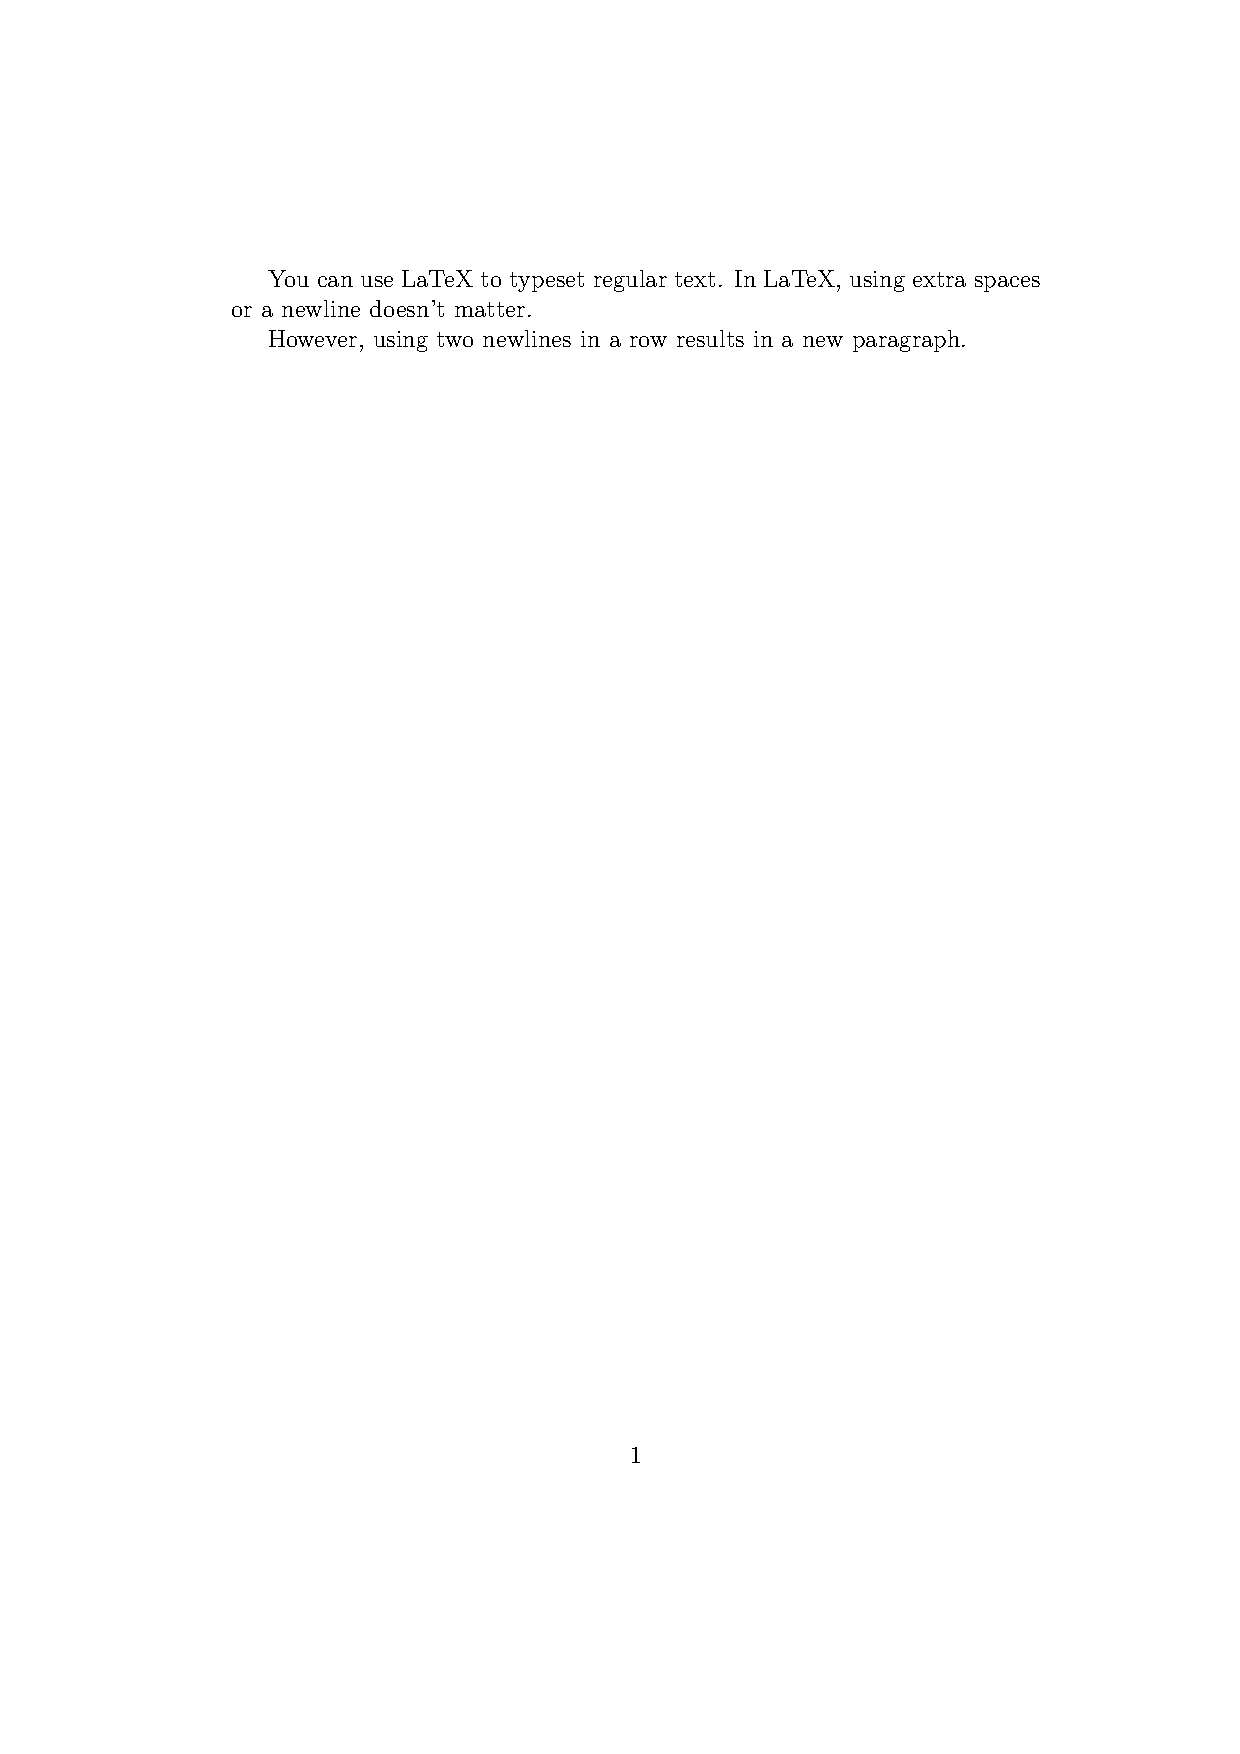
\includegraphics[trim = 33mm 230mm 33mm 40mm, clip, width=\textwidth]{figures/example_spacing.pdf}
  %\end{framed}
  \end{minipage}
\end{frame}

\begin{frame}[fragile]
  \frametitle{Cross-Referencing}
  \begin{itemize}
    \item Many things in \LaTeX{}, such as sections and subsections, are automatically numbered
    \begin{itemize}
      \item Numbering can be suppressed using asterisk, e.g.\ \verb|\section*{...}|
    \end{itemize}
    \item Automatically numbered entities in \LaTeX{} can be labeled using \verb|\label{...}|
    \item Any labeled entity can be referenced using \verb|\ref{...}|
    \item Command \verb|\ref{...}| is often preceded by \verb|~|, denoting a space that
      cannot be a line break
  \end{itemize}
  \begin{verbatim}\section{Introduction}
\label{sec:intro}
This is the introduction.
\section{Results}
In section~\ref{sec:intro}, we provided introductory
material. Now we will provide results.\end{verbatim}
\end{frame}

\begin{frame}[fragile]
  \frametitle{Compiling Multiple Times?}
  \begin{itemize}
    \item When running \verb|pdflatex| on \verb|example.tex|, multiple files are created
    \begin{itemize}
      \item \verb|example.pdf|: output file
      \item \verb|example.aux|: contains auxiliary about references, etc.
      \item \verb|example.log|, \verb|example.synctex.gz|, etc.
    \end{itemize}
    \item Cross-reference information in .aux file is not ready until
      after \verb|pdflatex| is run
    \begin{itemize}
      \item May need to run \verb|pdflatex| twice for references to display correctly
    \end{itemize}
    \item Using the tool LaTeX-Mk can resolve this issue
    \begin{itemize}
      \item Use command \verb|latexmk -pdf example.tex| to perform all operations needed to generate final pdf
    \end{itemize}
  \end{itemize}
\end{frame}

\frame{
  \frametitle{Exercise 1: Sections}
  \begin{itemize}
    \item Create the following document in \LaTeX{}
  \end{itemize}
  \centerline{
  \begin{minipage}{.6\textwidth} 
  \begin{framed}
    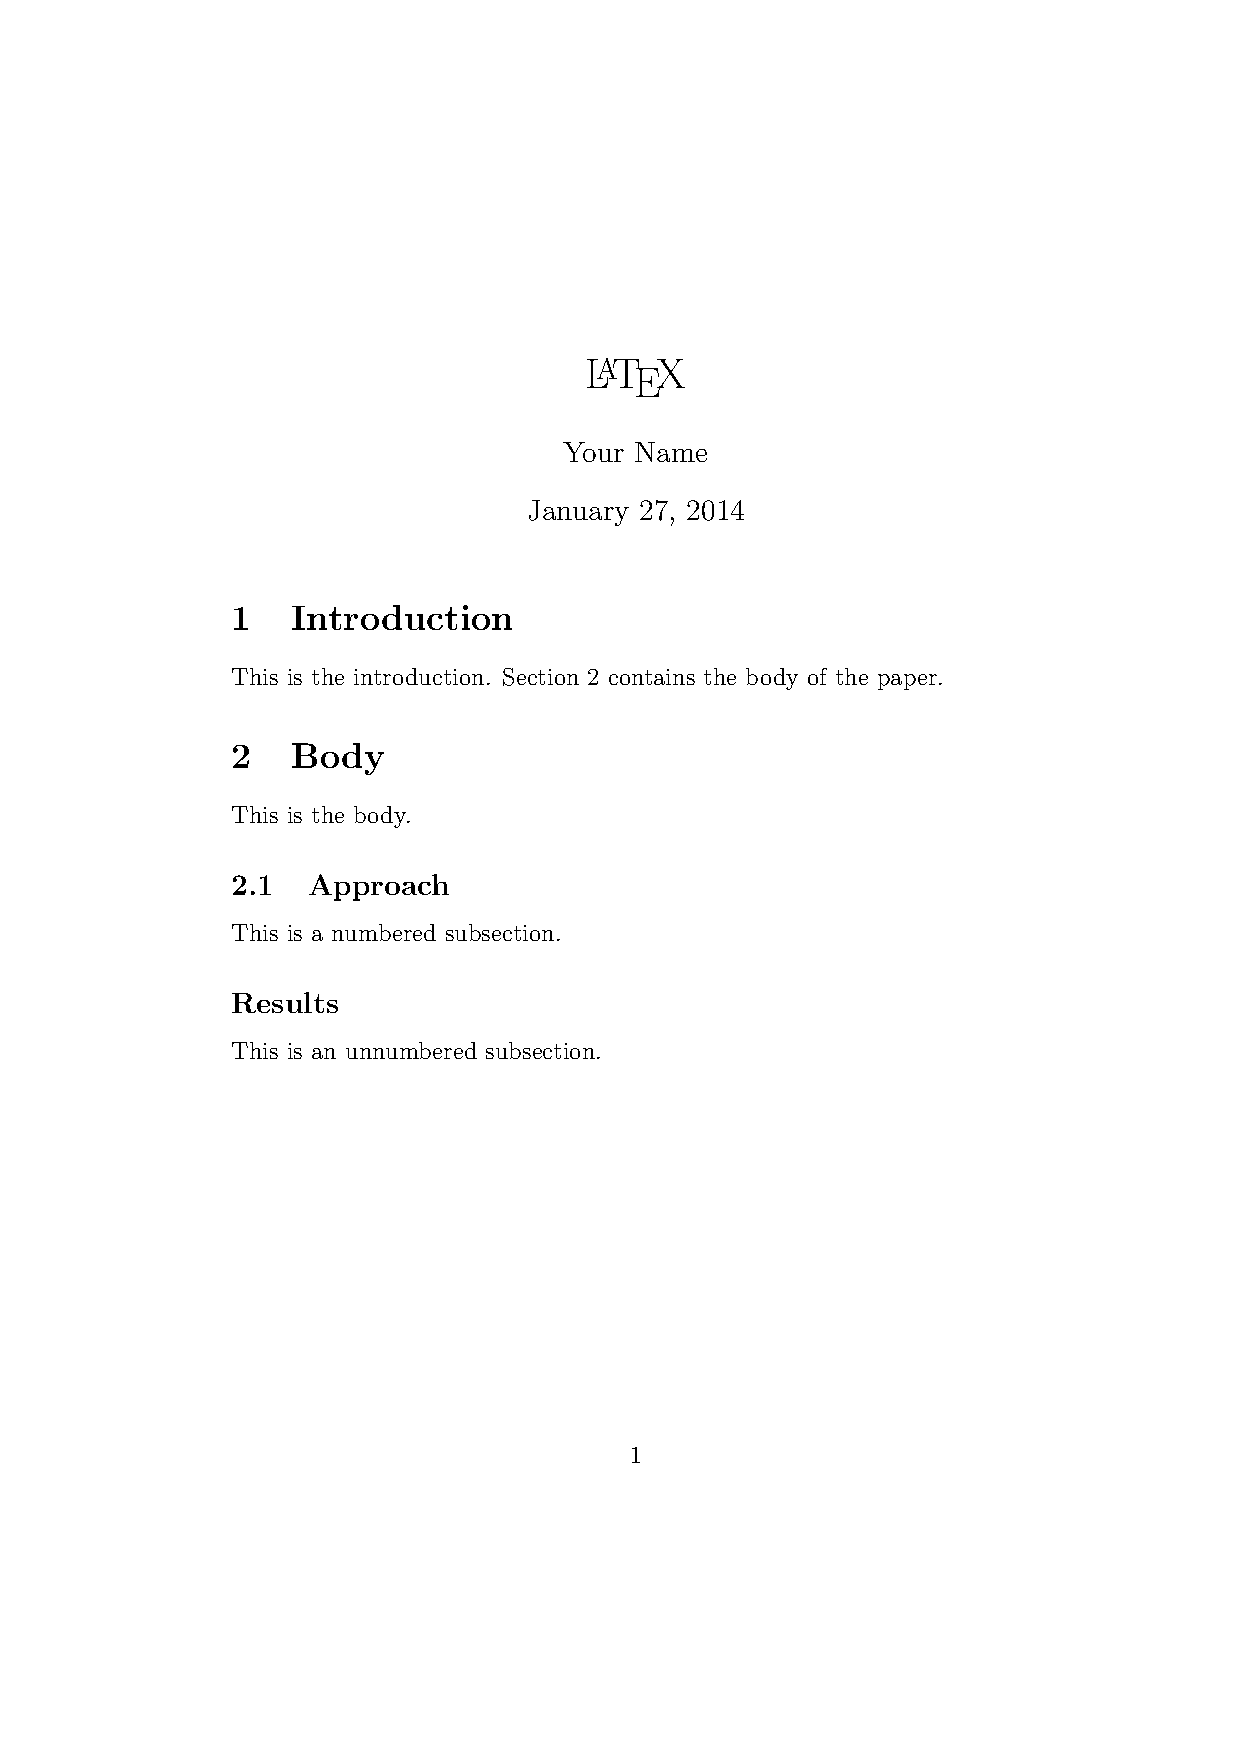
\includegraphics[trim = 33mm 115mm 33mm 59mm, clip, width=\textwidth]{figures/referencing.pdf}
  \end{framed}
  \end{minipage}
  }
  \begin{itemize}
    \item Helpful sites:
      \begin{itemize} \footnotesize
        \item http://en.wikibooks.org/wiki/LaTeX/Document\_Structure
        \item http://en.wikibooks.org/wiki/LaTeX/Labels\_and\_Cross-referencing
      \end{itemize}
  \end{itemize}
}

\begin{frame}[fragile]
  \frametitle{Exercise 1: Sections (Solution)}
{\small \begin{verbatim}\documentclass[12pt]{article}
\title{\LaTeX}
\author{Your Name}
\begin{document}
  \maketitle
  \section{Introduction}
  This is the introduction.  Section~\ref{sec:body} contains
  the body of the paper.
  \section{Body}
  \label{sec:body}
  This is the body.
    \subsection{Approach}
    This is a numbered subsection.
    \subsection*{Results}
    This is an unnumbered subsection.
\end{document}\end{verbatim} }
\end{frame}

\begin{frame}[fragile]
  \frametitle{Figures}
  \begin{itemize}
    \item Figures can be created using the figure environment
    \item Various options for placing figures
    \begin{itemize}
      \item \verb|h|: here, approximately
      \item \verb|t|: top
      \item \verb|b|: bottom
      \item \verb|p|: on its own page with other such figures
      \item For example, \verb|begin{figure}[ht]...| will place the figure
        approximately where it is listed in the markup and at the top of a page
    \end{itemize}
    \item Figures can include a caption and be labeled
  \end{itemize}
\end{frame}

\begin{frame}[fragile]
  \frametitle{Figures}
  \begin{itemize}
    \item The figure below was made with the following code:
  \end{itemize}
  \begin{verbatim}\begin{figure}
  \includegraphics[width=.6\textwidth]{siebel.jpg}
  \label{fig:siebel}
  \caption{A picture of Siebel Center}
\end{figure}\end{verbatim}
  \begin{figure}
     \includegraphics[width=.6\textwidth]{figures/siebel.jpg}
     \label{fig:siebel}
     \caption{A picture of Siebel Center}
  \end{figure}
  \scriptsize (image: cs.illinois.edu/sites/default/files/images/pagebanners/cropped-aboutus.jpg)
\end{frame}

\begin{frame}[fragile]
  \frametitle{BibTeX}
  \begin{itemize}
    \item BibTeX is a tool used to cite articles/books and automatically form a bibliography
    \item Use \verb|cite| command to cite something in your paper
    \begin{itemize} \item Example: \verb|\cite{greenwade93}| \end{itemize}
    \item Use \verb|\bibliographystyle| and \verb|\bibliography| commands at the
      end of document where bibliography should be
    \begin{itemize}
      \item Example: \verb|\bibliographystyle{plain}|  \verb|\bibliography{references}|
    \end{itemize}
    \item Make a .bib file (called references.bib in our example) that describes each source
  \end{itemize}
\end{frame}

\begin{frame}[fragile]
  \frametitle{BibTeX}
  \begin{itemize}
    \item Example .bib file:
  \end{itemize}
{\footnotesize  \begin{verbatim}@article{greenwade93,
    author  = "George D. Greenwade",
    title   = "The {C}omprehensive {T}ex {A}rchive {N}etwork
              ({CTAN})",
    year    = "1993",
    journal = "TUGBoat",
    volume  = "14",
    number  = "3",
    pages   = "342--351"
}
@book{goossens93,
    author    = "Michel Goossens and Frank Mittelbach and
                 Alexander Samarin",
    title     = "The LaTeX Companion",
    year      = "1993",
    publisher = "Addison-Wesley",
    address   = "Reading, Massachusetts"
}\end{verbatim} }
\end{frame}

\begin{frame}[fragile]
  \frametitle{Math Mode}
  \begin{itemize}
    \item Text between dollar signs \verb|$...$| will use math mode
    \item Many control sequences only work in math mode
    \item Can use \verb|^| for superscripts and \verb|_| for subscripts
  \end{itemize}
  \begin{table}
  \begin{tabular}{l l}
    \verb|$y = 3x - 4$| & $\rightarrow \quad y = 3x - 4$ \\
    \verb|$\theta \Theta \omega \Omega$| & $\rightarrow \quad \theta \Theta \omega \Omega$\\
    \verb|$\sqrt{x} = x^{1/2}$| & $\rightarrow \quad \sqrt{x} = x^{1/2}$\\
    \verb|$\min \{ x_1, x_2, x_3 \}$| & $\rightarrow \quad \min \{ x_1, x_2, x_3 \}$
  \end{tabular}
  \end{table}
\end{frame}

\begin{frame}[fragile]
  \frametitle{Displayed Math}
  \begin{itemize}
    \item Example: {\small \verb|f(x) = \sum_{i=1}^{\infty} \frac{1}{g_i(x)}|}
    \item Use dollar signs \verb|$...$| for inline math
      \begin{itemize} \item The equation $f(x) = \sum_{i=1}^{\infty} \frac{1}{g_i(x)}$ is displayed inline \end{itemize}
    \item Use escaped brackets \verb|\[...\]| to display math on its own line
      \[ f(x) = \sum_{i=1}^{\infty} \frac{1}{g_i(x)} \]
    \item Use \verb|\begin{equation}...\end{equation}| for automatically numbered equations
      \begin{equation} f(x) = \sum_{i=1}^{\infty} \frac{1}{g_i(x)} \end{equation}
  \end{itemize}
\end{frame}

\begin{frame}[fragile]
  \frametitle{Exercise 2: Definition of Derivative}
  \begin{itemize}
    \item Produce the following equation in \LaTeX{}:
    \[ \frac{\mathrm{d}f(x)}{\mathrm{d}x} = \lim_{\delta \to 0} \frac{f(x + \delta) - f(x)}{\delta} \]
    \item Start from the following:
  \end{itemize}
\begin{verbatim}\documentclass[11pt]{article}
\usepackage{amsmath}
\begin{document}
  % add your content here
\end{document}\end{verbatim}
  \begin{itemize}
    \item Helpful sites:
      \begin{itemize}
        \item en.wikibooks.org/wiki/LaTeX/Mathematics
        \item ftp.ams.org/pub/tex/doc/amsmath/short-math-guide.pdf
      \end{itemize}
  \end{itemize}
\end{frame}

\begin{frame}[fragile]
  \frametitle{Exercise 2: Definition of Derivative (Solution)}
  \begin{itemize}
    \item Produce the following equation in \LaTeX{}:
    \[ \frac{\mathrm{d}f(x)}{\mathrm{d}x} = \lim_{\delta \to 0} \frac{f(x + \delta) - f(x)}{\delta} \]
    \item Solution:
  \end{itemize}
  {\small \begin{verbatim}\[
  \frac{\mathrm{d}f(x)}{\mathrm{d}x}
  = \lim_{\delta \to 0} \frac{f(x + \delta) - f(x)}{\delta}
\]\end{verbatim}}
  \begin{itemize}
    \item Do the $\mathrm{d}$s in your solution look different?
      \begin{itemize} \item \verb|\mathrm| displays upright characters in math mode \end{itemize}
  \end{itemize}
\end{frame}

\begin{frame}[fragile]
  \frametitle{Array-Like Environments}
  \begin{itemize}
    \item Use \verb|array| environment or one of the matrix environments to make table of information
    \item Matrix environments include delimiters for convenience
    \begin{itemize}
      \item \verb|pmatrix| $()$, \verb|bmatrix| $[]$, \verb|Bmatrix| $\{\}$,
      \verb|vmatrix| $| |$, \verb|Vmatrix| $\| \|$
    \end{itemize}
    \item Columns separated with \verb|&|, rows separated with \verb|\\|
%    \item Column alignment specified at start using \verb|l| for left, \verb|c| for center
%      and \verb|r| for right
%   \begin{itemize}\item Example: \verb|{ccc}| means use three centered columns\end{itemize}
  \end{itemize}

  \begin{minipage}{.47\textwidth}
  \begin{framed}
    \begin{verbatim}A = \begin{pmatrix}
      2  & -1 & 0  \\
      -1 & 2  & -1 \\
      0  & -1 & 2
    \end{pmatrix}\end{verbatim}
  \end{framed}
  \end{minipage}
  $\rightarrow$
  \begin{minipage}{.43\textwidth} 
  \begin{framed}
    \[
%      A = \left( \begin{array}{ccc}
%      2 & -1 & 0 \\
%      -1 & 2 & -1 \\
%      0 & -1 & 2 \end{array} \right)
A = \begin{pmatrix}
      2  & -1 & 0  \\
      -1 & 2  & -1 \\
      0  & -1 & 2
    \end{pmatrix}
    \]
  \end{framed}
  \end{minipage}
\end{frame}

\begin{frame}[fragile]
  \frametitle{Align Environment}
  \begin{itemize}
    \item Use \verb|align| environment to line up multiple equations
    \item Left and right sides of equation separated with \verb|&|
    \item Equations separated with \verb|\\|
    \item Using \verb|align*| instead of \verb|align| will suppress equation numbers
  \end{itemize}
  \begin{minipage}{.52\textwidth}
  \begin{framed}
    \begin{verbatim}\begin{align}
  x & = \cos(\theta(t)) \\
  y & = \sin(\theta(t)) \\
  \theta(t) &
     = \omega t + \phi
\end{align}\end{verbatim}
  \end{framed}
  \end{minipage}
  $\rightarrow$
  \begin{minipage}{.41\textwidth} 
  \begin{framed}
    \begin{align}
      x & = \cos(\theta(t)) \\
      y & = \sin(\theta(t)) \\
     \theta(t) & = \omega t + \phi
    \end{align}
  \end{framed}
  \end{minipage}
\end{frame}

\begin{frame}[fragile]
  \frametitle{Resizing Delimiters}
  \begin{itemize}
    \item The \verb|\left|, \verb|\right|, and \verb|\middle| commands are used to automatically resize
      delimiters like parenthesis based on content
    \item Period \verb|.| denotes an omitted left or right delimiter
    \item The \verb|\big|, \verb|\Big|, \verb|\bigg|, and \verb|\Bigg| commands can be used to manually resize delimiters
  \end{itemize}
  \begin{table}
  \small
  \begin{tabular}{l l}
    \verb|$\left(\frac{x^2}{y+x}\right)^2$| & $\rightarrow \quad$ \begin{minipage}{.3\textwidth} \[ \left(\frac{x^2}{y + x}\right)^2 \]\end{minipage} \\
    \begin{minipage}{.6\textwidth}\begin{verbatim}$P\left(X=1 \middle|
  \frac{X}{Y} \geq 2 \right)$\end{verbatim}\end{minipage} & $\rightarrow \quad$ \begin{minipage}{.3\textwidth} \[ P\left(X=1 \middle|\frac{X}{Y} \geq 2\right) \]\end{minipage} \\
    \verb!$\left.2x-\frac{2}{x^3}\right|_0^1$! & $\rightarrow \quad$ \begin{minipage}{.3\textwidth}\[ \left.2x - \frac{2}{x^3}\right|_0^1\] \end{minipage} \\
    \verb|$( \big( \Big( \bigg( \Bigg($| & $\rightarrow \quad$ \begin{minipage}{.3\textwidth}\[ ( \big( \Big( \bigg( \Bigg( \] \end{minipage} 
  \end{tabular}
  \end{table}
\end{frame}

\begin{frame}[fragile]
  \frametitle{Math Accents}
  \begin{itemize} \item Special accents over variables/expressions may be used in math mode \end{itemize}
  \begin{table}
  \begin{tabular}{l l l l}
    \verb|$\bar{x}$| & $\rightarrow \quad \bar{x}$ &
    \qquad \qquad \verb|$\vec{x}$| & $\rightarrow \quad \vec{x}$ \\
    \verb|$\dot{x}$| & $\rightarrow \quad \dot{x}$ &
    \qquad \qquad \verb|$\hat{x}$| & $\rightarrow \quad \hat{x}$ \\
    \verb|$\ddot{x}$| & $\rightarrow \quad \ddot{x}$ &
    \qquad \qquad \verb|$\tilde{x}$| & $\rightarrow \quad \tilde{x}$ \\
    \verb|$\acute{x}$| & $\rightarrow \quad \acute{x}$ &
    \qquad \qquad \verb|$\grave{x}$| & $\rightarrow \quad \grave{x}$
  \end{tabular}
  \end{table}
\end{frame}

\begin{frame}[fragile]
  \frametitle{Exercise 3: More Math}
  \begin{itemize}
    \item Produce the following equations in \LaTeX{}:
      \begin{align*}
        \begin{vmatrix}a & b \\ c & d\end{vmatrix} & = ad - bc \\
        \hat{x}_i & = x_i \left(\sum_{j=0}^\infty x_j \right)^{-1}
      \end{align*}
    \item Be sure to include \verb|\usepackage{amsmath}|
    \item Helpful sites:
      \begin{itemize}
        \item en.wikibooks.org/wiki/LaTeX/Mathematics
        \item ftp.ams.org/pub/tex/doc/amsmath/short-math-guide.pdf
      \end{itemize}
  \end{itemize}
\end{frame}

\begin{frame}[fragile]
  \frametitle{Exercise 3: More Math (Solution)}
  \begin{itemize}
    \item Produce the following equations in \LaTeX{}:
      \begin{align*}
        \begin{vmatrix}a & b \\ c & d\end{vmatrix} & = ad - bc \\
        \hat{x}_i & = x_i \left(\sum_{j=0}^\infty x_j \right)^{-1}
      \end{align*}
    \item Solution:
  \end{itemize}
  {\small \begin{verbatim}\begin{align*}
  \begin{vmatrix} a & b \\ c & d \end{vmatrix} & = ad - bc \\
  \hat{x}_i & = x_i \left(\sum_{j=0}^\infty x_j \right)^{-1}
\end{align*}\end{verbatim}}
\end{frame}

\frame{
  \frametitle{If You Want to Know More \ldots}
  \begin{itemize}
    \item \emph{en.wikibooks.org/wiki/LaTeX/} \\ Excellent reference for \LaTeX{} in general
    \begin{itemize}
    \item \emph{en.wikibooks.org/wiki/LaTeX/Macros} \\ Reference for defining your own
      macros in \LaTeX{}
    \item \emph{en.wikibooks.org/wiki/LaTeX/Presentations} \\ Reference for making \LaTeX{}
      presentations using Beamer package
    \end{itemize}
    \item \emph{ftp.ams.org/pub/tex/doc/amsmath/short-math-guide.pdf} \\
      Useful summary of features for writing mathematics
    \item \emph{www.ctan.org} \\ CTAN stands for the Comprehensive \TeX{} Archive Network,
      and contains many standard \LaTeX{} packages
  \end{itemize}
}

\end{document}

\end{document}
